\documentclass[]{book}
\usepackage{lmodern}
\usepackage{amssymb,amsmath}
\usepackage{ifxetex,ifluatex}
\usepackage{fixltx2e} % provides \textsubscript
\ifnum 0\ifxetex 1\fi\ifluatex 1\fi=0 % if pdftex
  \usepackage[T1]{fontenc}
  \usepackage[utf8]{inputenc}
\else % if luatex or xelatex
  \ifxetex
    \usepackage{mathspec}
  \else
    \usepackage{fontspec}
  \fi
  \defaultfontfeatures{Ligatures=TeX,Scale=MatchLowercase}
\fi
% use upquote if available, for straight quotes in verbatim environments
\IfFileExists{upquote.sty}{\usepackage{upquote}}{}
% use microtype if available
\IfFileExists{microtype.sty}{%
\usepackage{microtype}
\UseMicrotypeSet[protrusion]{basicmath} % disable protrusion for tt fonts
}{}
\usepackage{hyperref}
\hypersetup{unicode=true,
            pdftitle={Similitud de Comunidades biológicas},
            pdfauthor={Carlos Iván Espinosa},
            pdfborder={0 0 0},
            breaklinks=true}
\urlstyle{same}  % don't use monospace font for urls
\usepackage{natbib}
\bibliographystyle{apalike}
\usepackage{longtable,booktabs}
\usepackage{graphicx,grffile}
\makeatletter
\def\maxwidth{\ifdim\Gin@nat@width>\linewidth\linewidth\else\Gin@nat@width\fi}
\def\maxheight{\ifdim\Gin@nat@height>\textheight\textheight\else\Gin@nat@height\fi}
\makeatother
% Scale images if necessary, so that they will not overflow the page
% margins by default, and it is still possible to overwrite the defaults
% using explicit options in \includegraphics[width, height, ...]{}
\setkeys{Gin}{width=\maxwidth,height=\maxheight,keepaspectratio}
\IfFileExists{parskip.sty}{%
\usepackage{parskip}
}{% else
\setlength{\parindent}{0pt}
\setlength{\parskip}{6pt plus 2pt minus 1pt}
}
\setlength{\emergencystretch}{3em}  % prevent overfull lines
\providecommand{\tightlist}{%
  \setlength{\itemsep}{0pt}\setlength{\parskip}{0pt}}
\setcounter{secnumdepth}{5}
% Redefines (sub)paragraphs to behave more like sections
\ifx\paragraph\undefined\else
\let\oldparagraph\paragraph
\renewcommand{\paragraph}[1]{\oldparagraph{#1}\mbox{}}
\fi
\ifx\subparagraph\undefined\else
\let\oldsubparagraph\subparagraph
\renewcommand{\subparagraph}[1]{\oldsubparagraph{#1}\mbox{}}
\fi

%%% Use protect on footnotes to avoid problems with footnotes in titles
\let\rmarkdownfootnote\footnote%
\def\footnote{\protect\rmarkdownfootnote}

%%% Change title format to be more compact
\usepackage{titling}

% Create subtitle command for use in maketitle
\providecommand{\subtitle}[1]{
  \posttitle{
    \begin{center}\large#1\end{center}
    }
}

\setlength{\droptitle}{-2em}

  \title{Similitud de Comunidades biológicas}
    \pretitle{\vspace{\droptitle}\centering\huge}
  \posttitle{\par}
    \author{Carlos Iván Espinosa}
    \preauthor{\centering\large\emph}
  \postauthor{\par}
      \predate{\centering\large\emph}
  \postdate{\par}
    \date{Noviembre 2018}

\usepackage{booktabs}

\begin{document}
\maketitle

{
\setcounter{tocdepth}{1}
\tableofcontents
}
\chapter*{Prefacio}\label{prefacio}
\addcontentsline{toc}{chapter}{Prefacio}

\begin{center}\rule{0.5\linewidth}{\linethickness}\end{center}

La comunidad biológica se refiere a una agrupación de poblaciones de
especies que se presentan juntas en el espacio y el tiempo (Begon et al.
1999). Este concepto plantea que las comunidades tienen unos límites
espaciales y temporales. Estos límites están dados por la distribución
de las poblaciones a lo largo de un gradiente espacial o temporal. De
esta forma los cambios en abundancia de las especies a lo largo de
gradientes espaciales o temporales generan la zonación y la sucesión
respectivamente.

La identificación de formaciones biológicas en el espacio
(\textbf{zonación}) o las etapas seriales a lo largo del tiempo
(\textbf{sucesión}) implica que tenemos la capacidad de establecer en
qué momento una comunidad cambia. Parece una tarea sencilla, pero
realmente no lo es, ¿cuánto debería cambiar una comunidad para poder
hablar de etapas seriales o zonas distintas? y ¿cómo podemos calcular
ese cambio? Una de las formas de responder estas preguntas puede ser
intentar cuantificar las similitudes entre localidades.

\chapter*{Objetivos}\label{objetivos}
\addcontentsline{toc}{chapter}{Objetivos}

\begin{center}\rule{0.5\linewidth}{\linethickness}\end{center}

En este ejercicio mostramos las bases del cálculo de similitud y
distancia entre comunidades, el cual se convierte en la base de los
análisis multivariantes de la comunidad.

Específicamente nos interesa;

\begin{itemize}
\tightlist
\item
  Comprender las bases teóricas para el cálculo de similitudes y
  distancias en la comunidad entre localidades.
\item
  Desarrollar mediciones de similitud entre localidades e interpretar
  los resultados.
\end{itemize}

\begin{figure}[htbp]
\centering
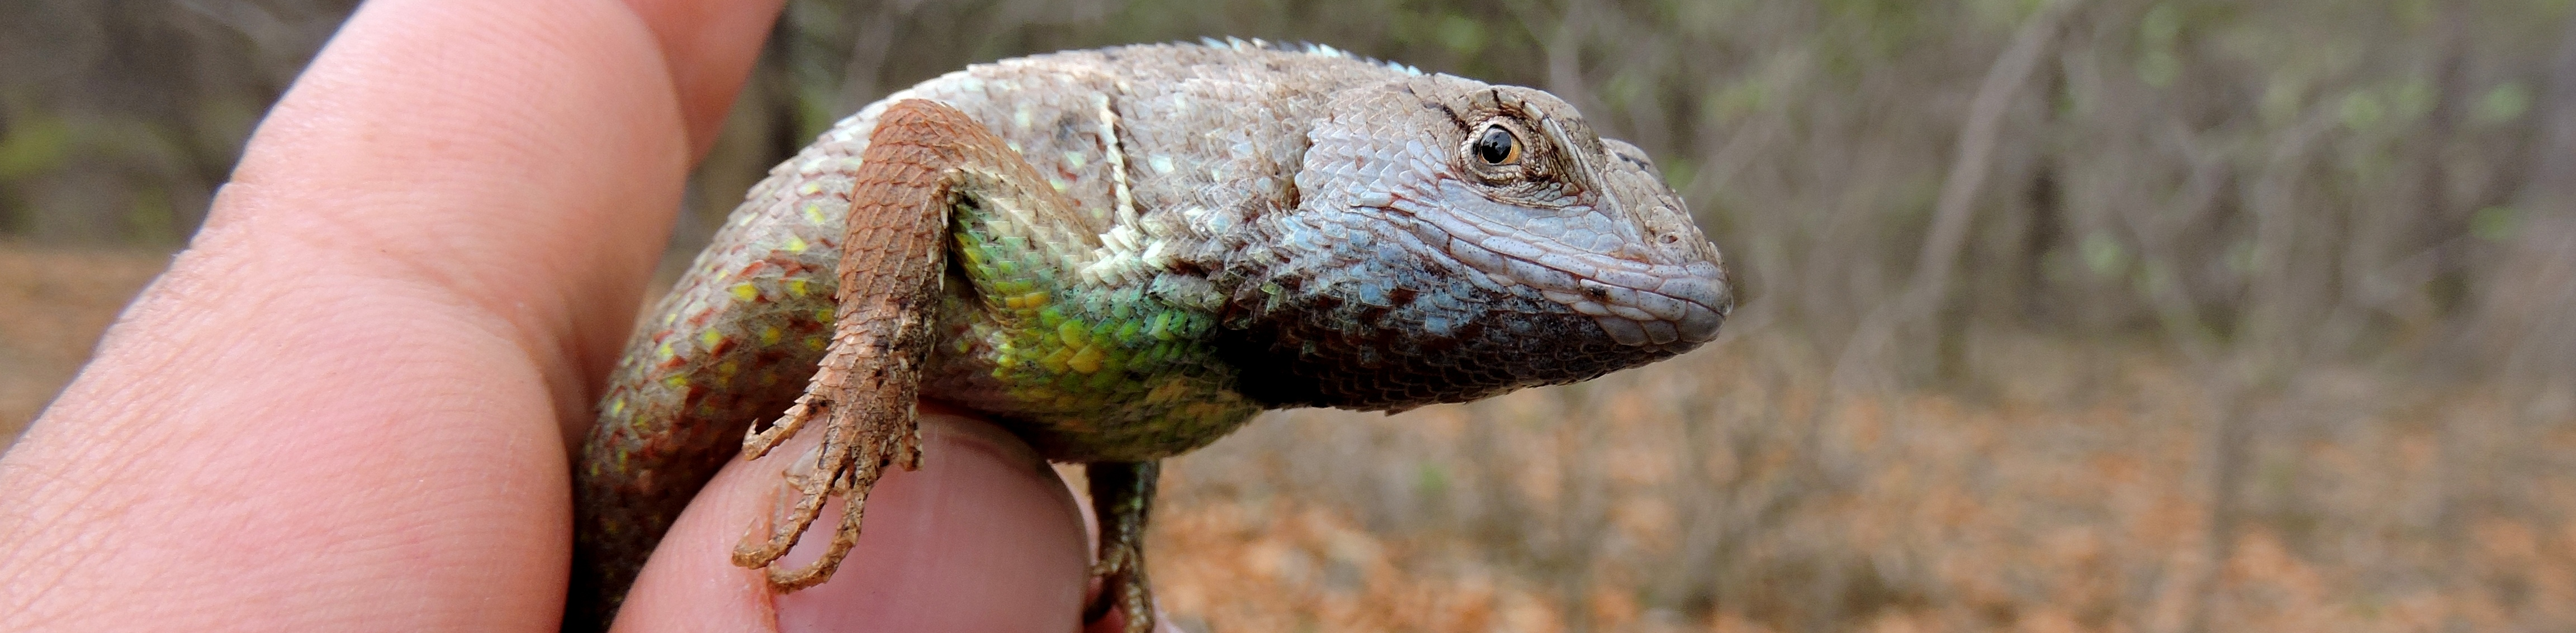
\includegraphics{lagar.jpg}
\caption{\emph{Stenocercus iridicens}}
\end{figure}

\chapter{Introducción}\label{introduccion}

Placeholder

\bibliography{packages.bib}


\end{document}
